\section{Auswertung}
\label{sec:Auswertung}
\subsection{Untersuchung des Acrylblocks mit dem A-Scan}
Im ersten Versuchsteil soll ein Acrylblock mit dem A-Scan untersucht werden. Die Messung der Probekörper mit einer Schieblehre beträgt die folgenden aufgeführten Werte:
\begin{align*}
b &= \SI{4}{\cm} \\
l &= \SI{15}{\cm} \\
h &= \SI{8}{\cm}.
\end{align*}
Dabei sind $b$ die Breite, $l$ die Länge und $h$ die Höhe der Probekörper. Dabei wird die Gleichung \ref{eq:time} angewendet und entsprechend nach $t$ umgestellt:
\begin{equation}
\label{eq:zeit}
t = \frac{2 \cdot s}{c}.
\end{equation}
Die Messwerte, die berechneten Laufzeiten und die Dicke der Fehlstellen $d$ befinden sich in der Tabelle \ref{tab:ascan}.  Für den A-Scan ist die Abbildung \ref{fig:2} zu sehen.

Die Dicke der Fehlstellen $d$ werden nach der folgenden Gleichung berechnet:
\begin{equation}
d = h - s_1 - s_2,
\end{equation}
wobei $s_1$ die jeweiligen Abstände für den nicht-umgedrehten Acrylblock und $s_2$ die jeweiligen Abstände für den umgedrehten Acrylblock sind.

\begin{table}[htpb]
	\centering
	\caption{Messwerte für den A-Scan.}
	\label{tab:ascan}
	\begin{tabular}{c c c c}
		\toprule
		$\text{Lochnummer}$ & $s_1/ \SI{e-3}{\meter} $& $s_2/ \SI{e-3}{\meter} $ & $d / \SI{e-3}{\meter}$ \\
		\midrule
		3 & 62   & 14,1 & 3,9 \\
		4 & 54,8 & 22,6 & 2,6 \\
		5 & 47,2 & 31,0 & 1,8 \\
		6 & 39,7 & 39,8 & 0,5 \\
		7 & 31,7 & 47,8 & 0,5 \\
		8 & 23,8 & 55,7 & 0,5 \\
		9 & 15,7 & 63,6 & 0,7 \\
		10 & 7,9 &  -   & - \\
		\bottomrule
	\end{tabular}
\end{table}

\begin{figure}[h!]
	\centering
	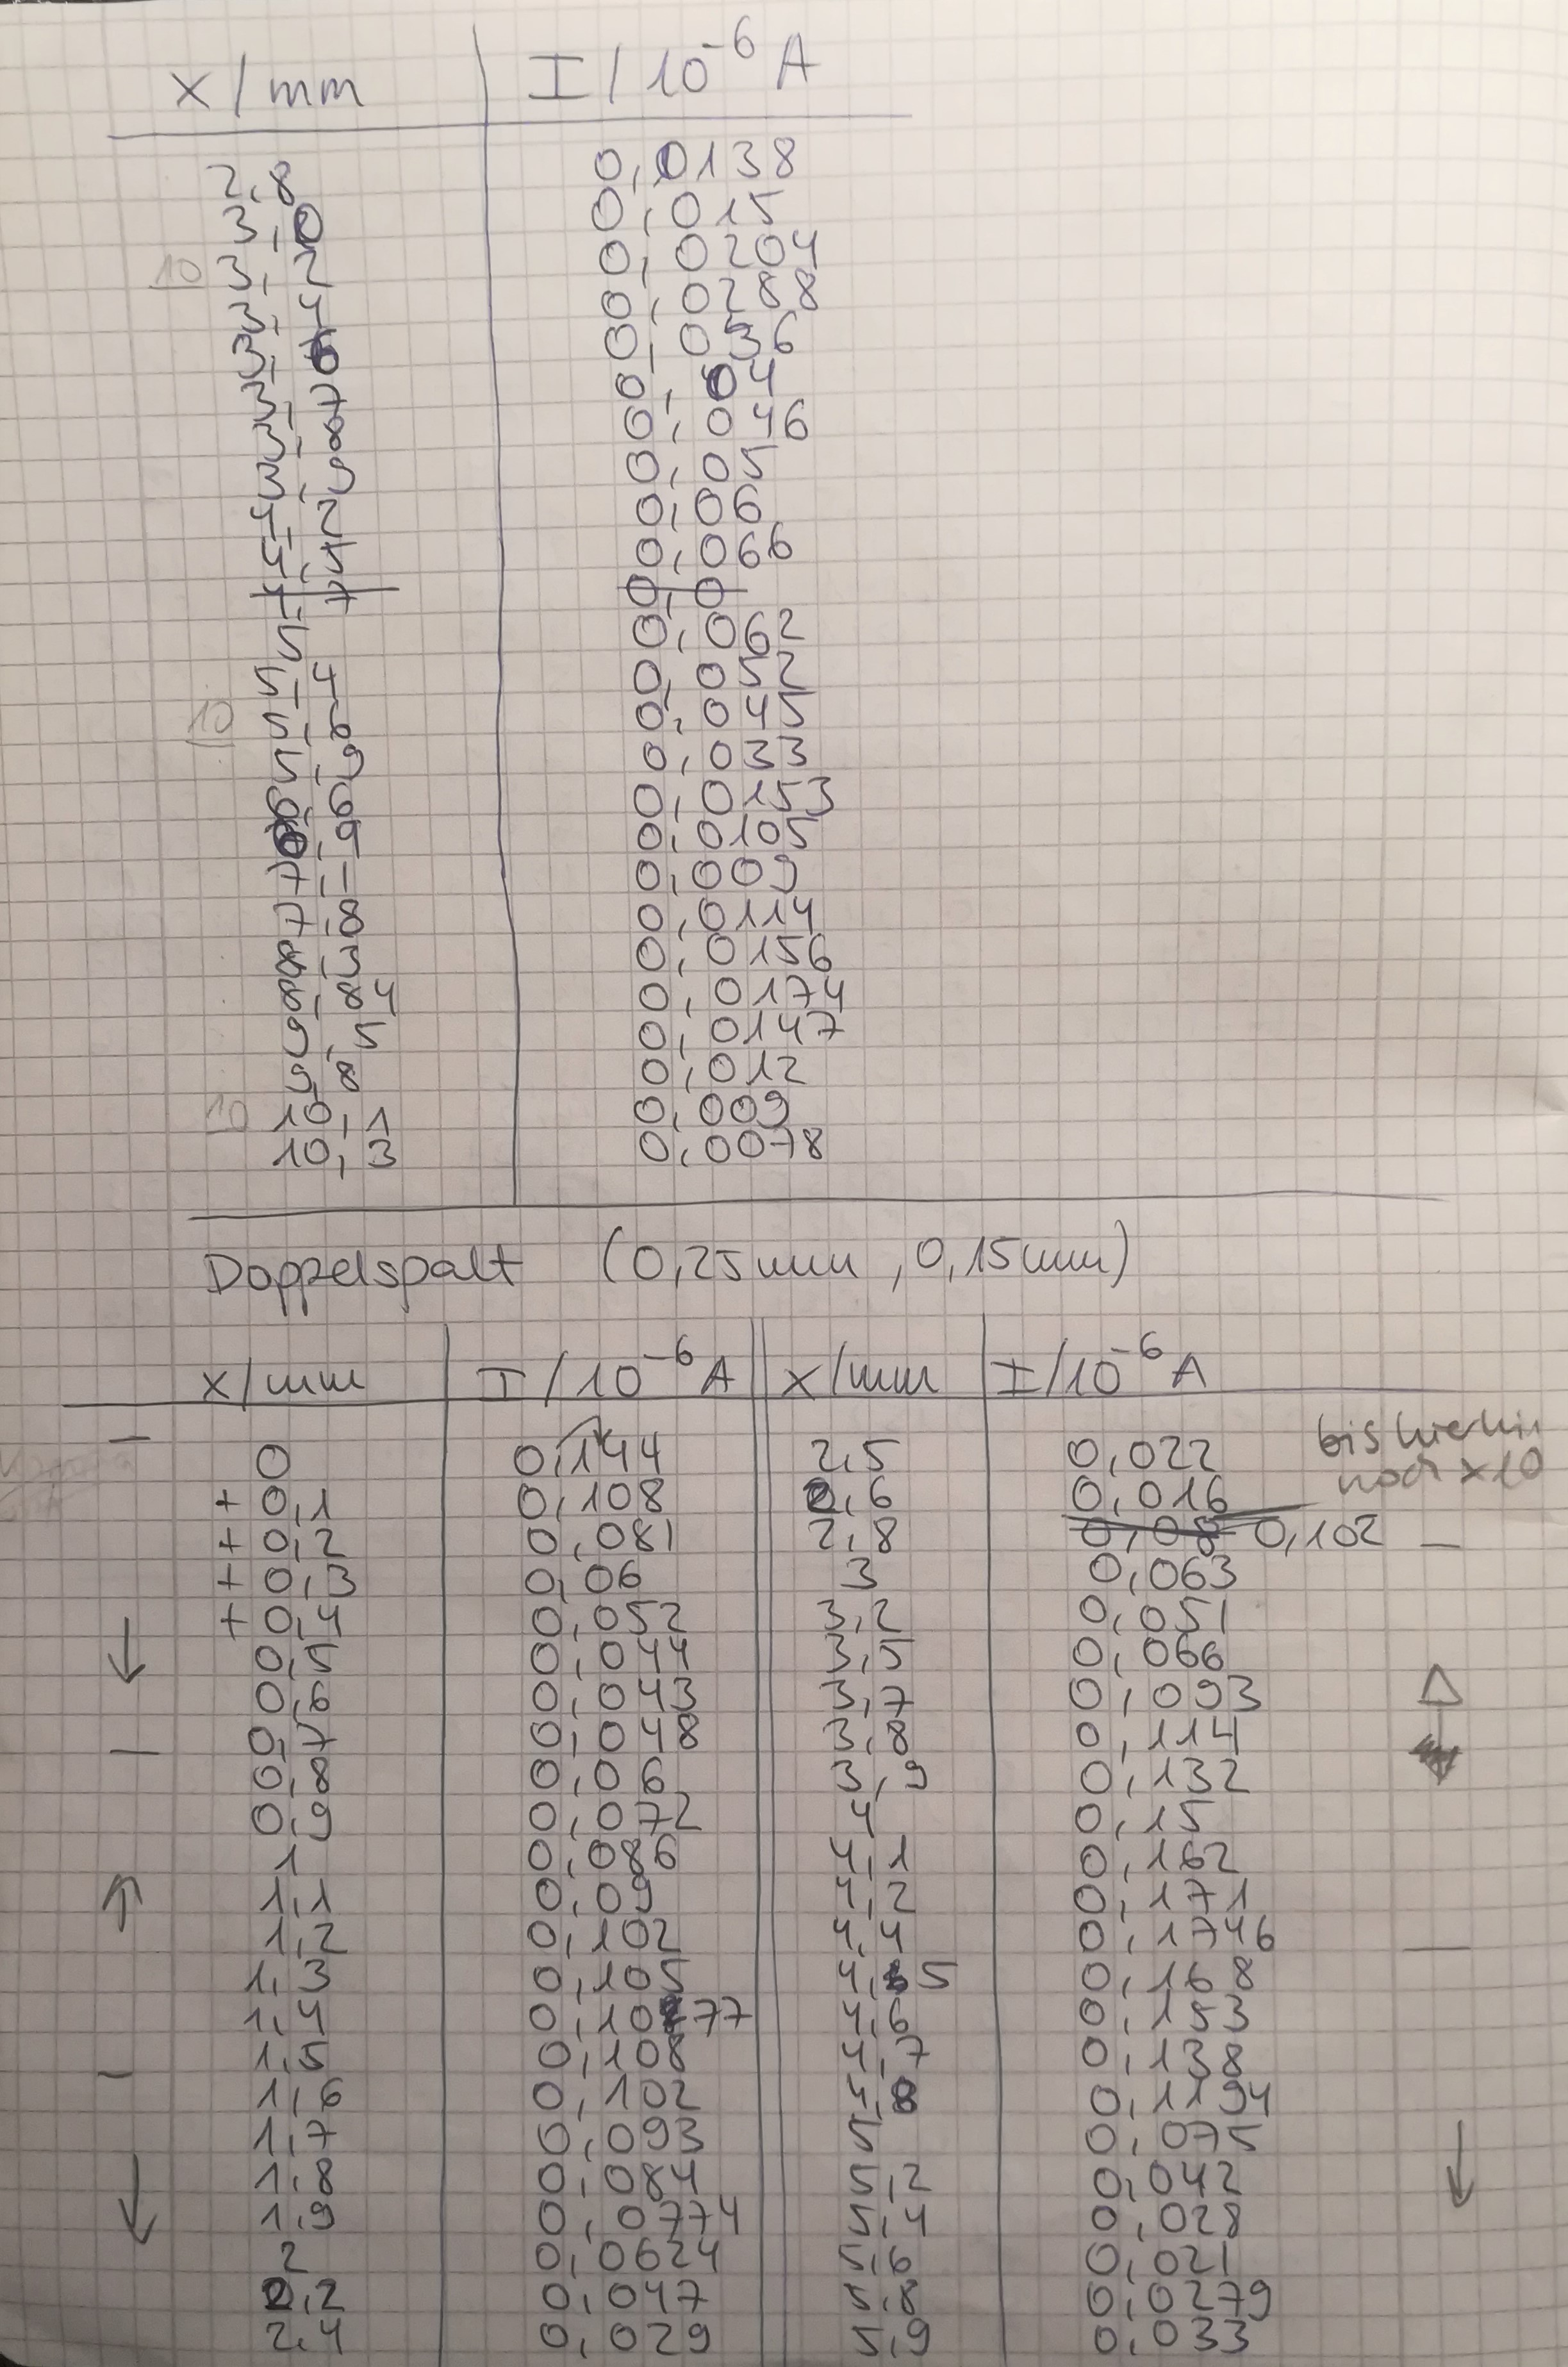
\includegraphics[width=0.7\linewidth]{../../2}
	\caption{Untersuchung des Acrylblocks mit dem A-Scan, das erste Bild.}
	\label{fig:2}
\end{figure}


\subsection{Untersuchung des Auflösungsvermögens}
In diesem Versuchsteil sollte das Auflösungsvermögen untersucht werden. Dabei wird es mit einer roten Sonde auf einen Acrylblock untersucht, welcher mit zwei benachbarten Fehlstellen zur Verfügung stand.

Die Wellenlänge\cite{Wellenlänge} ist gegeben als:
\begin{equation}
\label{eq:wellenlänge}
\lambda = \frac{c}{f} = \frac{c}{T}
\end{equation}
wobei $f =\SI{2}{\mega\hertz}$ beträgt und $c$ die Schallgeschwindigkeit in Acryl ist.
Daraus ergibt sich für den Abstand der zwei benachbarten Fehlstellen beziehungsweise die Wellenlänge aus der Gleichung \ref{eq:wellenlänge}:
\begin{equation*}
\lambda = \SI{1,365}{\milli\meter}.
\end{equation*}
Die Signalauflösung zeigt eine Abhängigkeit von der Frequenz der Ultraschallwelle, d.h. je höher die Frequenz, um so besser die Auflösung, um so geringer aber die Eindringtiefe. Für eine niedrige Frequenz wie bei der roten Sonde mit $\SI{2}{\mega\hertz}$ ergibt sich eine geringe Auflösung aber eine große Eindringtiefe.
 
\subsection{Untersuchung des Acrylblocks mit dem B-Scan}

Für den selben Acrylblock mit verschiedenen Bohrungen wird nun mit dem B-Scan Verfahren ein zwei-dimensionales Bild des Blocks erstellt, auf dem die Bohrungen hervorgehoben sind. Dies wurde mit einer roten Sonde, die $\SI{2}{\mega\hertz}$ beträgt, durchgeführt. Dabei ergaben sich die Abbildungen \ref{fig:pic1} und \ref{fig:pic2} für eine nicht-umgedrehte als auch umgedrehte Lage. Als Schallgeschwindigkeit in Acryl wird der Literaturwert\cite{Velocities} verwendet. Für die Lochnummer $1,2,10$ konnten die Laufzeiten aufgrund der schwachen Darstellung für die beiden Lagen nicht abgelesen werden. Sie konnten nicht gemessen werden, während die anderen nahe Störstellen scharf dargestellt wurden.

\begin{figure}[h!]
	\centering
	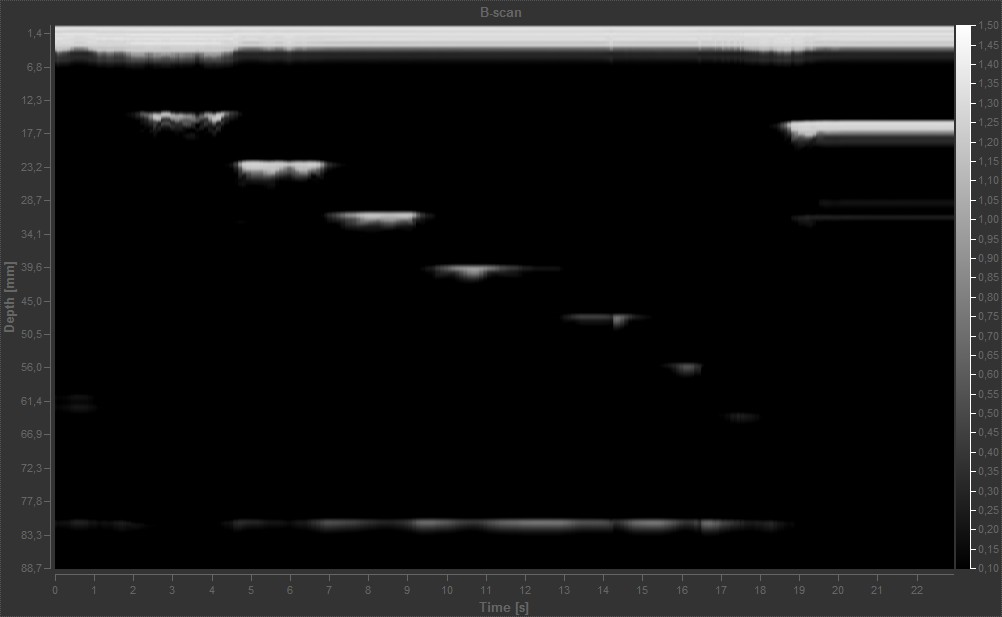
\includegraphics[width=0.7\linewidth]{../../pic1}
	\caption{Abbildung des Acrylblocks im B-Scan mit einer roten Sonde für eine umgedrehte Lage.}
	\label{fig:pic1}
\end{figure}

\begin{figure}[h!]
	\centering
	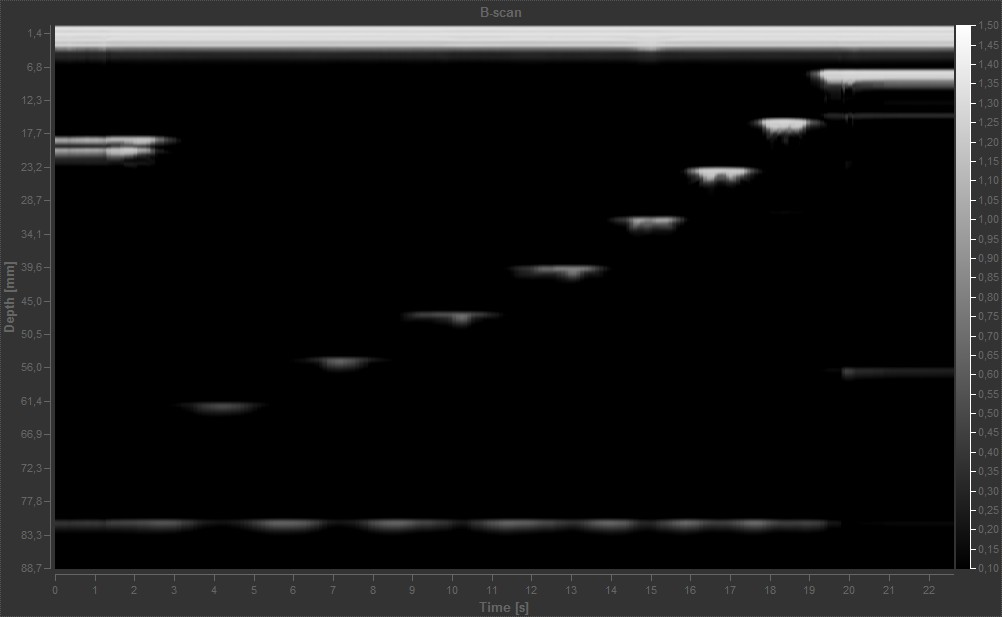
\includegraphics[width=0.7\linewidth]{../../pic2}
	\caption{Abbildung des Acrylblocks im B-Scan mit einer roten Sonde für eine nicht-umgedrehte Lage.}
	\label{fig:pic2}
\end{figure}
 
Die Abstände der Fehlstellen $s$ werden nach der folgenden Formel berechnet:
\begin{equation}
s = h - c \cdot \frac{t}{2},
\end{equation}
wobei $h$ die Höhe, $c$ die Schallgeschwindigkeit in Acryl und $t$ die jeweilige Laufzeit sind. Die Dicke der Fehlstellen $d$ ergibt sich dann, indem die jeweils von oben und unten gemessene Abstände vom Rand zur Bohrung abgezogen werden:
\begin{equation}
d = h - s_\text{oben} - s_\text{unten}.
\end{equation}

 Die Messwerte zu dem B-Scan sowie die daraus berechneten Fehlstellen $s$ und Dicken $d$ befinden sich in der Tabelle \ref{tab:bscan}. 

\begin{table}[htpb]
	\centering
	\caption{Messwerte zur Bestimmung der Lage und Dicke der Fehlstellen für den B-Scan.}
	\label{tab:bscan}
	\begin{tabular}{c c c c c c}
		\toprule
		$\text{Lochnummer}$ & $t_\text{oben} / \SI{e-6}{\second}$ & $t_\text{unten} / \SI{e-6}{\second}$ & $s_\text{oben} / \SI{e-3}{\meter}$ & $s_\text{unten} / \SI{e-3}{\meter}$ & $d / \SI{e-3}{\meter}$ \\
		\midrule
		3 & 14,2 & 17  & 19,38 & 23,24 & 3,74 \\
		4 & 22,2 & 24,7 & 30,3 & 33,72 & 1,6 \\  
		5 & 30,6 & 32,5 & 41,77 & 44,36 & 0,61 \\ 
		6 & 39,2 & 40,9 & 53,51 & 55,83 & 2,93 \\
		7 & 47,4 & 48,2 & 64,7 & 65,8 & 1,42 \\
		8 & 55,2 & 56,5 & 75,35 & 77,12 & 7,25 \\
		9 & 63,6 & 64,4 & 86,81 & 87,91 & 9,47 \\
		10 & 15,2 & 18,8 & 20,75 & 25,67 & 3,36 \\
		\midrule
		3 & 61,8 & 63,4 & 84,36 & 86,54 & 9,09 \\
		4 & 54,3 & 56,2 & 74,12 & 76,71 & 7,08 \\
		5 & 46,9 & 48,1 & 64,02 & 65,66 & 4,97 \\
		6 & 39,2 & 40,9 & 53,51 & 55,83 & 2,93 \\
		7 & 31,2 & 32,9 & 42,59 & 44,91 & 0,75 \\
		8 & 23,2 & 25,2 & 31,67 & 34,4 & 1,39 \\
		9 & 15,2 & 17,3 & 20,75 & 23,61 & 3,56 \\
		10 & 7,1 & 9,7  & 9,67 & 13,24 & 5,71 \\
		\bottomrule
	\end{tabular}
\end{table}

\subsection{Bestimmung des Herzzeitvolumens(HZV)}

Mit der Sonde soll ein einfaches Herzmodell untersucht und das entsprechende Herzzeitvolumen $\text{HZV}$ bestimmt werden. In der Abbildung \ref{fig:pic4} kann die Kurve zur Bestimmung des Herzvolumens in der TM-Mode angesehen werden. Zum einen ist die Gleichung \ref{eq:herzzeitvolumen} relevant, weil sie für die Berechnung des Herzzeitvolumens benötigt wird:
\begin{equation}
\label{eq:herzzeitvolumen}
\text{HZV} = (\text{EDS}-\text{EDV}) \cdot \nu_\text{Herz}
\end{equation}
wobei $\text{EDV}$ das enddiastolische Volumen, $\text{EDS}$ das endsystolische Volumen und $\nu_\text{Herz}$ die Herzfrequenz sind. Hierbei haben sich $10$ Schläge in $\SI{24}{\second}$ Sekunden ergeben, also es gilt:
\begin{equation*}
\label{eq:herzfreq}
\nu_\text{herz} = \frac{n}{T_\text{ges}} = \SI{0,41}{\hertz}
\end{equation*}
wobei $n$ die Anzahl der Schläge und $T$ die Gesamtanzahl der Sekunden sind. Es wird angenommen, dass das simulierte Herzmodell ein Kegelvolumen\cite{Kegelvolumen} besitzt, damit das endsystolische Volumen bestimmt werden kann. Das Volumen eines Kegel ist gegeben wie folgt:
\begin{equation}
\label{eq:kegelvol}
V_\text{Kegel} = \frac{1}{3} \cdot A \cdot h = \frac{1}{3} \cdot \pi \cdot r^{2} \cdot h 
\end{equation}
und in Gleichung \ref{eq:kegelvol} wird für die Fläche $A$ die Formel für eine Kreisfläche eingesetzt und damit ergibt sich:
\begin{equation}
\label{eq:kegelkreis}
V_\text{Kegel} = \frac{1}{3} \cdot (\frac{\pi}{4} \cdot D^{2}) \cdot h =  \frac{1}{12} \cdot \pi \cdot D^{2} \cdot h,
\end{equation}
wobei $D$ der Membrandurchmesser, welcher $D = \SI{0,046}{\meter}$ beträgt und $h$ die Höhe für welche $\text{EDS}$ eingesetzt wird. Für die Berechnung des endsystolischen Volumens werden die Werte aus der Tabelle \ref{tab:herzzeitvol} übernommen und damit ergibt sich $\text{EDS} = \SI{0,085}{\meter}$. Die Werte für den Membrandurchmesser $D$ und den endsystolischen Volumen $\text{EDS}$ werden in die Gleichung \ref{eq:kegelkreis} eingesetzt und es ergibt sich ein Wert von:
\begin{equation*}
V_\text{Kegel} = \text{EDV} = \SI{47}{\cubic\cm}.
\end{equation*}
Dann werden die Werte für die Herzfrequenz und für den enddiastolische Volumen in die Gleichung \ref{eq:herzzeitvolumen} eingesetzt und daraus folgt für das Herzzeitvolumen:
\begin{equation*}
\text{HZV} = \SI{19,27}{\frac{\milli\liter}{\second}} = \SI{1,15}{\frac{\liter}{\minute}}.
\end{equation*}

\begin{table}[htpb]
	\centering
	\caption{Messwerte zur Bestimmung des HZV.}
	\label{tab:herzzeitvol}
	\begin{tabular}{c c c}
		\toprule
		$D / \si{\cm}$ & $h_1 / \si{\milli\meter}$ & $h_2 / \si{\milli\meter}$ \\
		\midrule
		4,6 & 19,1 & 27,6 \\
		\bottomrule
	\end{tabular}
\end{table}

\begin{figure}[h!]
	\centering
	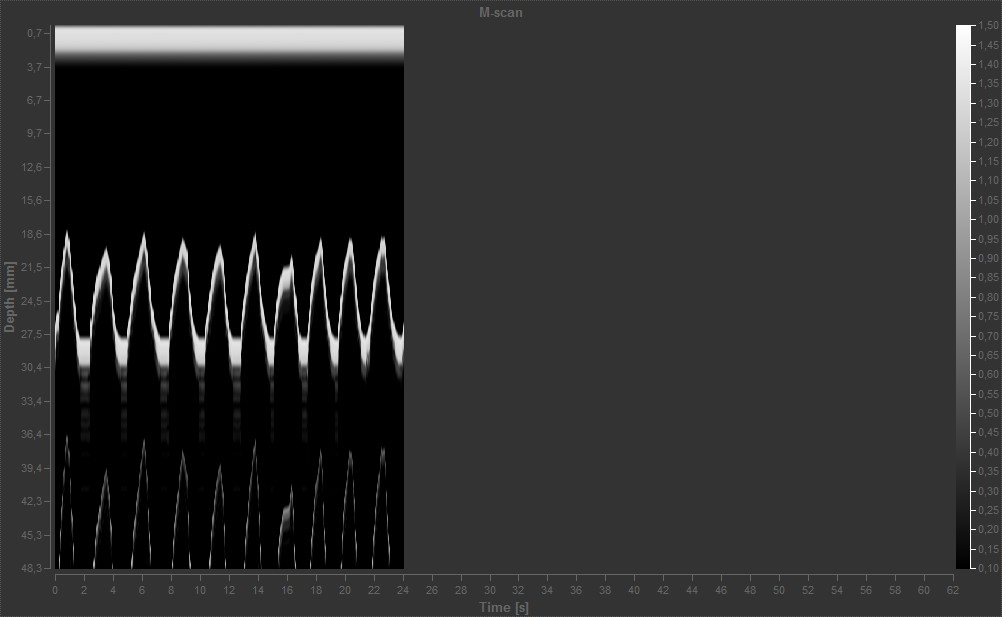
\includegraphics[width=0.7\linewidth]{../../pic4}
	\caption{TM-Mode zur Bestimmung des Herzzeitvolumens.}
	\label{fig:pic4}
\end{figure}
